\documentclass{article}
\usepackage{graphicx}
\usepackage{geometry}
\usepackage{amsmath}

%%%%%%%%%%%%%%%%%%%%%%%%%%%%%%%%%%%%%%%%

\DeclareMathOperator*{\vectorize}{vec}

\newcommand{\normal}[2]{\ensuremath{\mathcal{N}\left({{#1}},{{#2}}\right)}}
\newcommand{\trans}[1]{\ensuremath{{#1}^{\mathsf{T}}}}

\newcommand{\e}{\mathbf{e}}
\newcommand{\bb}{\mathbf{b}}
\newcommand{\w}{\mathbf{w}}
\newcommand{\x}{\mathbf{x}}
\newcommand{\y}{\mathbf{y}}
\newcommand{\uu}{\mathbf{u}}
\newcommand{\vv}{\mathbf{v}}

%%%%%%%%%%%%%%%%%%%%%%%%%%%%%%%%%%%%%%%%%%%%%%%%%%%%%%%%%%%%%%%%%%%%%%%%%%%%%%%%

\begin{filecontents}{paper.bib}
@inproceedings{wan2000unscented,
  title={The unscented Kalman filter for nonlinear estimation},
  author={Wan, Eric A and Van Der Merwe, Rudolph},
  booktitle={Adaptive Systems for Signal Processing, Communications, and Control Symposium 2000. AS-SPCC. The IEEE 2000},
  pages={153--158},
  year={2000},
  organization={Ieee}
}

@article{wang2010generating,
  title={Generating statistically correct random topologies for testing smart grid communication and control networks},
  author={Wang, Zhifang and Scaglione, Anna and Thomas, Robert J},
  journal={IEEE transactions on Smart Grid},
  volume={1},
  number={1},
  pages={28--39},
  year={2010},
  publisher={IEEE}
}
\end{filecontents}
\immediate\write18{bibtex paper}

%%%%%%%%%%%%%%%%%%%%%%%%%%%%%%%%%%%%%%%%%%%%%%%%%%%%%%%%%%%%%%%%%%%%%%%%%%%%%%%%

\begin{document}

%%%%%%%%%%%%%%%%%%%%%%%%%%%%%%%%%%%%%%%%

\section{The problem}
%\subsection{Control theory statement}
We are given a dynamical system defined by the following state equation.
\begin{align}
\label{sys:orig}
\x_{t+1} &= (A + B_t)\x_t + C(\uu_t + \vv_t) + \epsilon,~~~~~ \epsilon \sim \normal{0}{P}
%\x_{t+1} &= (A + B_t)\x_t + C\uu_t + \epsilon ,~~~~~ \epsilon \sim \normal{0}{P}
\end{align}
We assume that matrices $A$ and $C$ are fixed in advance and known;
the matrix $B_t$ is time dependent, unknown, and set adversarily;
state variable $\x_t$ is observed at each iteration with error $\epsilon$;
the input $\uu_t$ is the control signal present during normal system operation;
and the input $\vv_t$ is an unobserved control signal set adversarily.
The adversary manipulates $B_t$ and $\uu_t$ to add positive feedback to the system with the goal of destabilizing it.
Our goal is to determine which states are subject to positive feedback so that we can take corrective action to restore stability.

\subsection{Partially observed control}

In the case of the power grid problem,
we are also interested in the cases where the normal control inputs are either unobserved or observable only at a low frequency.
If we assume that $\uu$ follows a Gaussian random walk, then we have
\begin{equation}
\uu_t = \uu_{f(t)} + \nu_{t-f(t)}
,~~~~~ \nu_{t-f(t)} \sim \normal{0}{(t-f(t))Q}
\end{equation}
where $f(t)$ denotes the time of the most recent observation of $\uu$.

The resulting dynamical system is defined by
\begin{align}
\label{sys:orig}
\x_{t+1} &= (A + B_t)\x_t + C(\uu_{f(t)} + \vv_t) + \epsilon_t
,~~~~~ \epsilon_t \sim \normal{0}{P+(t-f(t))CQ}
\end{align}
For simplicity in the equations below, we do not perform this substitution.
In all the problems I've experimented with, the effect of fully observing the control $\uu_t$ versus not observing it at all is negligible.
The control signal must be very large and sporadic before adding the low frequency information is useful.

%\subsection{Power grid statement}

%%%%%%%%%%%%%%%%%%%%%%%%%%%%%%%%%%%%%%%%

\section{Proposed solution}
We can solve for the $B_t$ matrix directly by augmenting the dynamical system's state variables to include the elements of the matrix.
This technique is called dual state estimation.
The resulting augmented system is
\begin{align}
\begin{pmatrix}
\x_{t+1} \\
\vectorize B_{t+1}
\end{pmatrix}
=
\begin{pmatrix}
A + B_t \\
I
\end{pmatrix}
\begin{pmatrix}
\x'_t \\
\vectorize B_t
\end{pmatrix}
+
\begin{pmatrix}
C \\
I
\end{pmatrix}
\begin{pmatrix}
\uu_t + \vv_t \\
\w_t
\end{pmatrix}
+
\begin{pmatrix}
\epsilon \\
\nu
\end{pmatrix}
 ,~~~~~ \epsilon \sim \normal{0}{P}
 , \nu\sim\normal{0}{Q}
\end{align}
Here we have also introduced a new control input $\w_t$ with error $\nu$.
Like $\uu_t$, the $\w_t$ vector is unobserved and controlled by the attacker.
The attacker uses $\w_t$ to manipulate the $B_t$ matrix.
This system is no longer linear, but it can be solved using the Unscented Kalman Filter \cite{wan2000unscented}.

To make the model easier to solve, we use the following two simplifying assumptions.
\begin{enumerate}
\item
Since $\vv_t$ and $\w_t$ are unobserved,
we can model their contribution as random error terms.
Under the assumption that $\vv_t\sim\normal{0}{R}$ and $\w_t\sim\normal{0}{S}$, we get the system
\begin{align}
\begin{pmatrix}
\x_{t+1} \\
\vectorize B_{t+1}
\end{pmatrix}
=
\begin{pmatrix}
A + B_t \\
I
\end{pmatrix}
\begin{pmatrix}
\x'_t \\
\vectorize B_t
\end{pmatrix}
+
\begin{pmatrix}
C \\
I
\end{pmatrix}
\begin{pmatrix}
\uu_t \\
0
\end{pmatrix}
+
\begin{pmatrix}
\epsilon \\
\nu
\end{pmatrix}
 ,~~~~~ \epsilon \sim \normal{0}{P+R}
 , \nu\sim\normal{0}{Q+S}
\end{align}


\item
We only care about which states have positive feedback present (the rows of $B_t$);
we don't care about which states are contributing the positive feedback (the columns of $B_t$).
In the power grid problem, we also have that most state variables will have similar values (approximately zero) when the system is stable.
Therefore, we can factorize the attack matrix as $B_t \approx \trans\e\bb_t$ where $\e$ is the vector of all ones.
This results in the state equation
\begin{align}
\begin{pmatrix}
\x_{t+1} \\
\bb_t
\end{pmatrix}
=
\begin{pmatrix}
A + \trans\e\bb_t \\
I
\end{pmatrix}
\begin{pmatrix}
\x'_t \\
\bb_t
\end{pmatrix}
+
\begin{pmatrix}
C \\
0
\end{pmatrix}
\begin{pmatrix}
\uu_t + \w_t\\
\vv_t
\end{pmatrix}
+
\begin{pmatrix}
\epsilon \\
\nu
\end{pmatrix}
 ,~~~~~ \epsilon \sim \normal{0}{P}
 , \nu\sim\normal{0}{Q}
\end{align}
Making the value of $\e$ reflect the likely contributions of each source in a time dependent manner would likely improve the results.
\end{enumerate}

\section{Experiments}

I generated the power grids using the \emph{clusterSmallWorlds} model proposed by \cite{wang2010generating}.
The procedure is roughly to first generate a random number of ring shaped grids with $<10$ buses each;
then randomly add connections between the buses.
The article claims this accurately models the shape of realworld power networks up to about 300 buses.

One problem I'm encountering with scaling the problem sizes is that estimation of the $\bb$ parameters in unstable.
Consider the following system with 60 buses:
\begin{center}
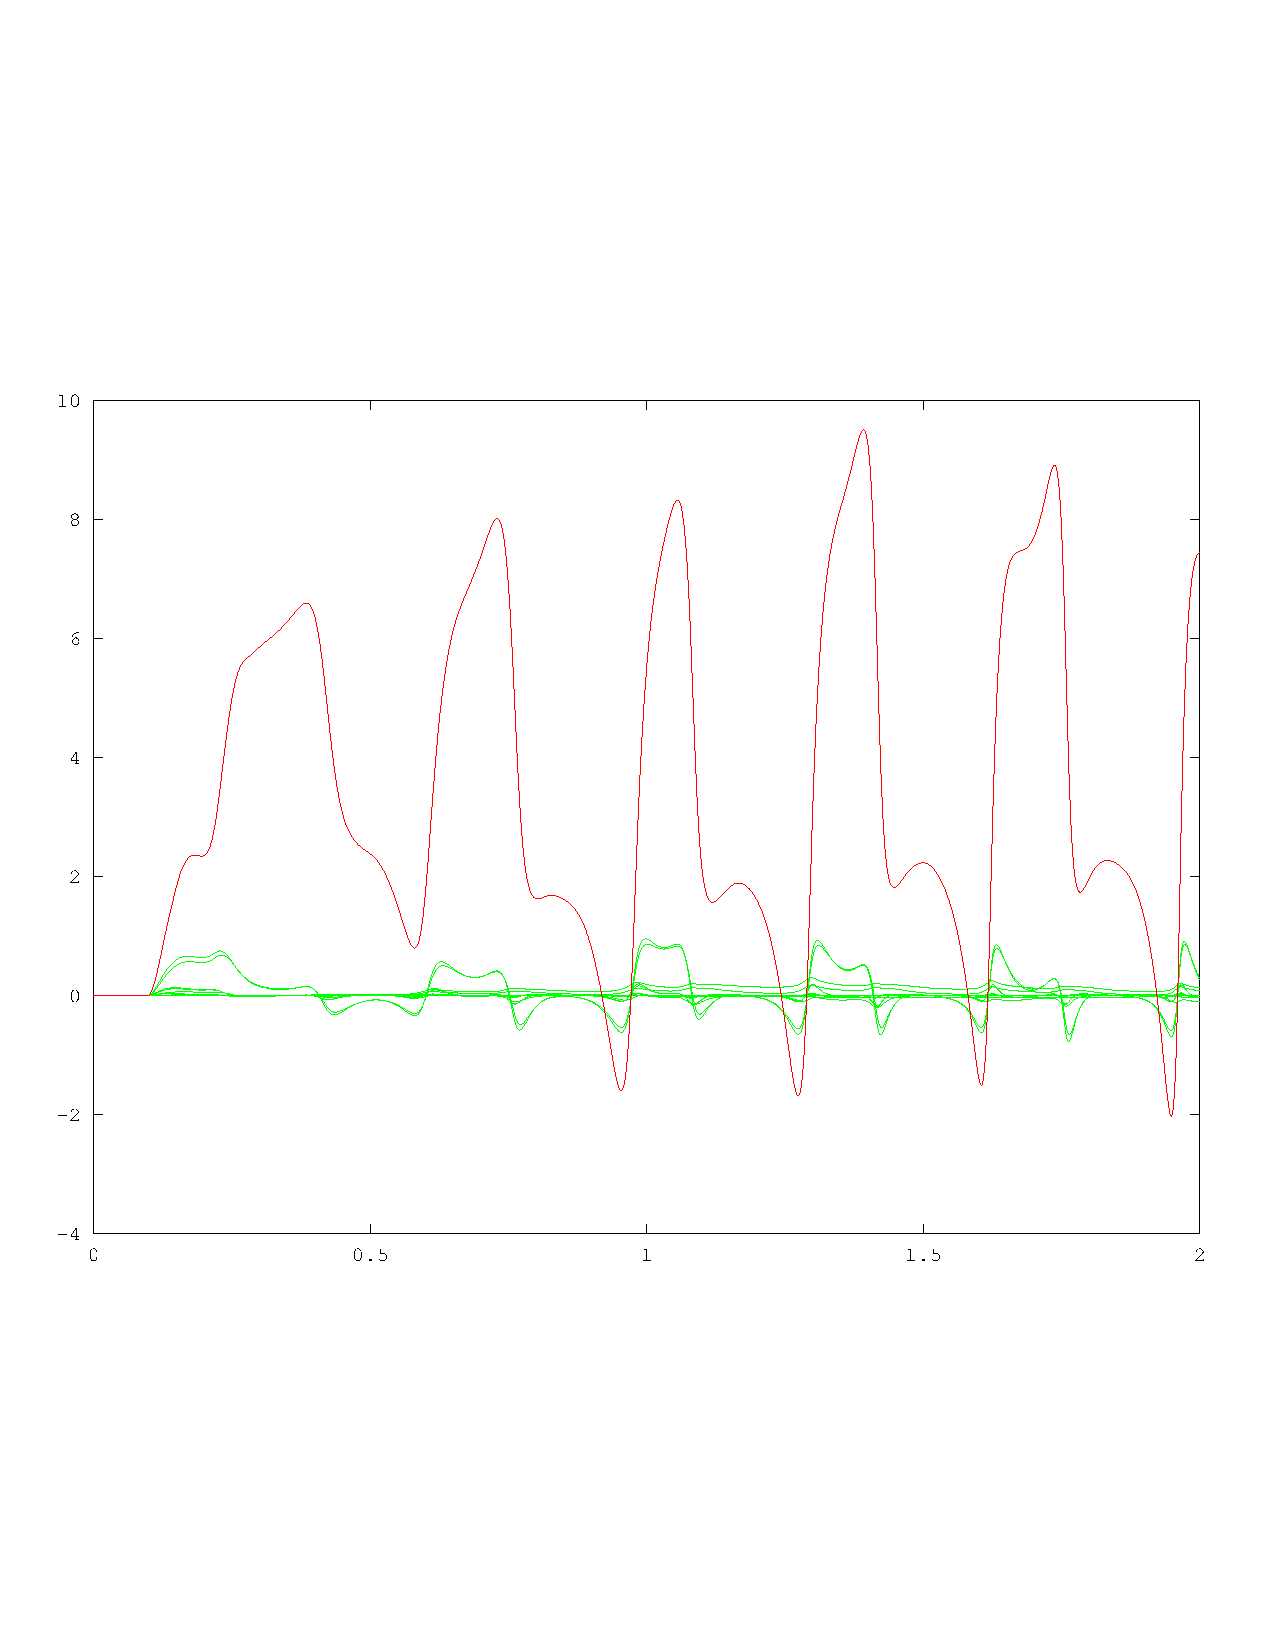
\includegraphics[width=0.6\textwidth,trim=0 2in 0 2in,clip]{img/ring-30-10-localSpike-gaussian-Observed-localKL-2-ukf}
\end{center}
The red lines indicate the attacked element of $\bb$ and the green lines the non-attacked elements.
As you can see, the estimates of the attack need to be damped somehow.

\bibliographystyle{plain}
\bibliography{paper}
\end{document}

